% !TEX root = main.tex

\section{多元函数的微分}
\subsection{微分}
偏导数的定义在此我们不再提及(即只将一个变量视为变量,其他变量视为常量),在本节中我们主要采用下面两种记号
\[f_x(x,y):=\pd{f(x,y)}{x}\qquad f_y(x,y):=\pd{f(x,y)}{y}\]
关于其他变元的偏导数采用类似的记法,之后不再赘述.
关于简单偏导数的求法在此也不再提及,关键选定主元,区别变量与常数.
\begin{definition}[全微分]
设函数$z=f(x,y)$在$P_0(x_0,y_0)$点的某邻域有定义,若函数在$P_0$的全改变量为
\[\begin{aligned}
\Delta z&:=f(x_0+\Delta x,y_0+\Delta y)-f(x_0,y_0)\\
&=A\Delta x+B\Delta y+o(\sqrt{(\Delta x)^2+(\Delta y)^2})
\end{aligned}\]
其中$A,B$为与$\Delta x,\Delta y$无关(可与$P_0$有关的常数),则称函数在$P_0$可微,其全微分为
\[\diff z\mid_{P_0}:=A\Delta x+B\Delta y\]
若$z$在$P_0$可微,则$f_x(x_0,y_0)$与$f_y(x_0,y_0)$均存在,
\[\diff z\mid_{P_0}=f_x(x_0,y_0)\diff x+f_y(x_0,y_0)\diff y\]
类似可定义$n$元函数$u=f(x_1,x_2,\ldots,x_n)$的全微分,
\[\diff u=\pd{u}{x_1}\diff x_1+\pd{u}{x_2}\diff x_2+\cdots+\pd{u}{x_n}\diff x_n\]
又由定义~\ref{def:multi_derivative_intro},
\[\lim_{\mathbf{h}\to \mathbf{0}}\frac{\|f(\mathbf{x}+\mathbf{h})-(f(\mathbf{x_0})+\mathbf{J}(\mathbf{x_0})\cdot \mathbf{h})\|_{\mathbb{R}^n}}{\|\mathbf{h}\|_{\mathbb{R}^m}}=0\]
其中$\mathbf{J}$为雅可比(Jacobian)矩阵
\[\mathbf{J}=\frac{\partial (y_1,\ldots,y_m)}{\partial (x_1,\ldots,x_n)}=\begin{bmatrix}
\pd{y_1}{x_1} & \cdots & \pd{y_1}{x_n}\\
\vdots & \ddots & \vdots\\
\pd{y_m}{x_1} & \cdots & \pd{y_m}{x_n}
\end{bmatrix}\]
特别地,对于二元函数
\[\mathbf{J}=\nabla f\implies \diff u=\nabla f\cdot\diff \vx\]
\end{definition}
直观地展示全微分,即为各个坐标方向上的增量乘上$\tan$切线夹角之和,见图\ref{fig:total_diff}
\begin{figure}[H]
\centering
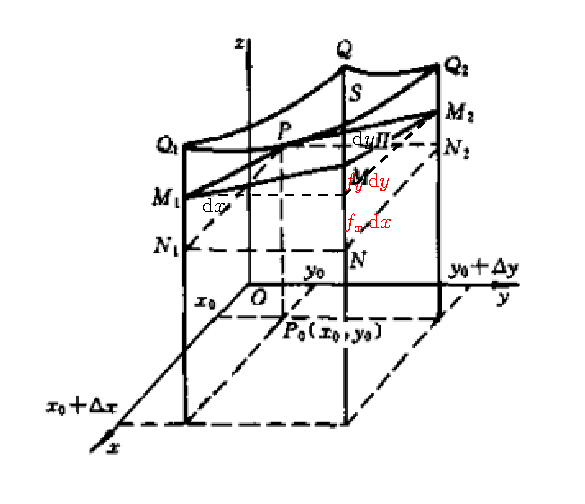
\includegraphics[width=0.4\linewidth]{fig/total_diff.eps}
\caption{全微分}
\label{fig:total_diff}
\end{figure}
\begin{theorem}
两个偏导数都连续$\implies$可微$\implies$连续
\end{theorem}
微分中值定理在多元微积分依然是利器,上述定理和下面的例题均可用其证明。
\begin{example}
设$u=f(x,y)$在矩形:$a<x<b$,$c<y<d$内可微,且全微分$\diff u$恒为$0$,证明$f(x,y)\equiv C$
\end{example}
\begin{analysis}
由全微分定义有
\[\diff u=f_x\diff x+f_y\diff y\equiv 0\]
推得
\[f_x=f_y\equiv 0\]
由微分中值定理
\[\begin{aligned}
f(x,y)-f(x_0,y_0)&=f(x,y)-f(x_0,y)+f(x_0,y)-f(x_0,y_0)\qquad\mbox{加一项减一项}\\
&=f_x(x_0+\theta_1(x-x_0),y)(x-x_0)+f_y(x,y_0+\theta_2(y-y_0))(y-y_0)\\
&=0\qquad\theta_1,\theta_2\in(0,1)
\end{aligned}\]
\end{analysis}
类似可证下例。
\begin{example}
设$f_x$在$(x_0,y_0)$存在,$f_y$在$(x_0,y_0)$存在,则$f(x,y)$在$(x_0,y_0)$连续
\end{example}
\begin{definition}[高阶偏导数]
以二阶为例,有以下四个偏导数,其中中间两个称为混合偏导数. 注意要将新偏导内容放最后
\[\begin{aligned}
\pdd{f}{x}&=\pd{}{x}\lrp{\pd{f}{x}}=f_{x^2}\\
\pddxy{f}{x}{y}&=\pd{}{y}\lrp{\pd{f}{x}}=f_{xy}\\
\pddxy{f}{y}{x}&=\pd{}{x}\lrp{\pd{f}{y}}=f_{yx}\\
\pdd{f}{y}&=\pd{}{y}\lrp{\pd{f}{y}}=f_{y^2}
\end{aligned}\]
\end{definition}
\begin{theorem}[混合偏导数相等]
若函数$f$具有直到$n$阶的连续偏导数,则求偏导数与变量的顺序无关,即
\[\pddd{n}{f}{x^k}{y^{n-k}}=\dfrac{\partial^n f}{\partial y\partial x^k\partial y^{n-k-1}}=\cdots=\pddd{n}{f}{y^{n-k}}{x^{k}}\]
\end{theorem}
$n$阶全微分是$(n-1)$阶全微分作为$x,y$函数的全微分
\par 注意$\diff x$、$\diff y$是自变量的微分,故视为常数,即
\[\diff(\diff x)=\diff(\diff y)=0\]
\begin{theorem}[高阶全微分]
当$n$阶偏导数连续时,
\[\begin{aligned}
\diff^n u&=\sum_{k=0}^n\binom{n}{k}\pddd{n}{f(x,y)}{x^{n-k}}{y^k}\diff x^{n-k}\diff y^k\\
&=\lrp{\pd{}{x}\diff x+\pd{}{y}\diff y}^n f(x,y)
\end{aligned}\]
这与二项式定理呈现的一样
\end{theorem}

\subsection{复合函数偏导数}
注意分清哪些量是自变量,哪些量是因变量,谁是谁的函数. 关键在于找好路径,将所有路径叠加即可. 分清究竟是不是复合函数. 建议在计算过程中采用更为简洁的$f_x,f_y$记法,方便计算
\begin{theorem}
若$u=f(x_1,x_2,\ldots,x_m)$在$(x_1,x_2,\ldots,x_m)$可微,$x_k(t_1,t_2,\ldots,t_n)$的所有偏导数存在,则复合函数
\[u=f(x_1(t_1,t_2,\ldots,t_n),\ldots,x_m(t_1,t_2,\ldots,t_n))\]
在$(t_1,t_2,\ldots,t_n)$的偏导数存在,为
\[\pd{u}{t_i}=\sum_{k=1}^m\pd{f}{x_k}\pd{x_k}{t_i}\]
简记为
\[u_{t_i}=f_{t_i}=\sum_{k=1}^n f_{x_k}(x_k)_{t_i}\]
\end{theorem}
\begin{example}
设$u=f(x,y),x=x(s,t),y=y(s,t)$都有连续的二阶偏导数,求复合函数$u(x(s,t),y(s,t))$的二阶偏导数$\disp\pdd{u}{s}$
\end{example}
\begin{analysis}
画出函数之间的关系图,红色标明的为两条含有$s$变元的路径
\[{\color{red}{f}}\Bigbr{{\color{red}{x}}\Bigbr{{\color{red}{s}}}{t}}{{\color{red}{y}}\Bigbr{{\color{red}{s}}}{t}}\]
故可得一阶偏导数
\[\pd{u}{s}=f_s=f_x x_s+f_y y_s\]
此时$f_x,f_y$均是关于$x,y$的函数,即
\[\textcolor{red}{f_x},\textcolor{red}{f_y}\Bigbr{\textcolor{red}{x}\Bigbr{\textcolor{red}{s}}{t}}{\textcolor{red}{y}\Bigbr{\textcolor{red}{s}}{t}}\]
进而
\[\begin{aligned}
\pdd{u}{s}&=f_{ss}=\pd{}{s}\lrp{\pd{u}{s}}\\
&=(f_x x_s)_s+(f_y y_s)_s\qquad\mbox{加法法则}\\
&=(f_x)_s x_s+x_{ss} f_x+(f_y)_s y_s+y_{ss}f_y\qquad\mbox{乘法法则}\\
&=(f_{xx}x_s+f_{xy}y_s)x_s+x_{ss}f_x+(f_{yx}x_s+f_{yy}y_s)y_s+y_{ss}f_y\qquad\mbox{链式法则}\\
&=f_{xx}(x_s)^2+2f_{xy}x_sy_s+f_{yy}(y_s)^2+x_{ss}f_x+y_{ss}f_y
\end{aligned}\]
\end{analysis}
二阶全微分不再具有形式不变性
\[\diff^2 u=\left[\pdd{f}{x}(\diff x)^2+2\pddxy{f}{x}{y}\diff x\diff y+\pdd{f}{y}(\diff y)^2\right]+\left[\pd{f}{x}\diff^2 x+\pd{f}{y}\diff^2 y\right]\]
常用于变量代换解偏微分方程,也有很多有趣的应用
\begin{example}
$z=f(x,y)$可微,在坐标旋转变换$x=u\cos\theta-v\sin\theta,y=u\sin\theta+v\cos\theta$下(其中旋转角$\theta$为常数),有\textbf{形式不变量}
\[\lrp{\pd{z}{x}}^2+\lrp{\pd{z}{y}}^2\]
\end{example}

\subsection{隐函数偏导数}
与一元的时候一样,将谁视为谁的函数,则需要用链式法则进行求导;但需要分清是否是复合函数,不是复合则直接用导数运算法则即可
\begin{example}
$u=f(x+ut,y-ut)$求$u$关于$t$的偏导数
\end{example}
\begin{analysis}
法一:\\
设隐函数$u=g(x,y,t)$,令$a=x+ut,b=y-ut$,则
\[\textcolor{red}{f}\Bigbr{a=x+ut=x+g(x,y,t)t=\textcolor{red}{a}(x,y,t)\begin{cases}x\\y\\\textcolor{red}{t}\end{cases}}{b=y-ut=y-g(x,y,t)t=\textcolor{red}{b}(x,y,t)\begin{cases}x\\y\\\textcolor{red}{t}\end{cases}}\]
一定要分清哪些是复合函数,哪些不是. 如上式$f$与$a,b$是复合函数关系,故要用链式法则;而$a,b$与$x,y,t$并不是复合,而仅仅是等式关系.
同时也要分清哪些是自变量,哪些是因变量,如上式的$u$是因变量,真正的自变量是$x,y,t$
\[\begin{aligned}
u_t&=(f(a,b))_t\\
&=f_a a_t+f_b b_t\qquad\mbox{链式法则}\\
&=f_a (x+ut)_t + f_b (y-ut)_t\qquad\mbox{代入等式}\\
&=f_a (u_t t+u)- f_b (u_t t+u)\qquad\mbox{乘法法则}\\
\end{aligned}\]
移项整理可得
\[u_t=\dfrac{(f_a-f_b)u}{1-t(f_b-f_a)}\]
法二:由一阶微分形式不变性\\
\[\begin{aligned}
\diff u&=f_a\diff(x+ut)+f_b\diff(y-ut)\\
&=f_a(\diff x+t\diff u+u\diff t)+f_b(\diff y-t\diff u-u\diff t)
\end{aligned}\]
进而
\[\diff u=\frac{f_a\diff x+f_b\diff y+u(f_a-f_b)\diff t}{1+t(f_b-f_a)}\]
\end{analysis}
对于隐函数组的情况,则相当于解一个线性方程组
\begin{example}
极坐标变换$x=r\cos\theta,y=r\sin\theta$,求$r,\theta$关于$x,y$的一阶偏导数
\end{example}
\begin{analysis}
法一:
\[\begin{cases}
x=r\cos\theta\\
y=r\sin\theta
\end{cases}\]
对上式左右两边同时对$x$求偏导数,有
\[\begin{cases}
F(r,\theta)=r_x\cos\theta-r\sin\theta\cdot\theta_x-1=0\\
G(r,\theta)=r_x\sin\theta+r\cos\theta\cdot\theta_x=0
\end{cases}\]
即
\[\begin{bmatrix}F_r&F_\theta\\G_r&G_\theta\end{bmatrix}
\begin{bmatrix}r_x\\\theta_x\end{bmatrix}
=\begin{bmatrix}F_x\\G_x\end{bmatrix}
=\begin{bmatrix}1\\0\end{bmatrix}\]
可求得雅可比行列式
\[J=\pd{(F,G)}{(r,\theta)}=\vmat{F_r&F_\theta\\G_r&G_\theta}
=\vmat{\cos\theta & -r\sin\theta\\\sin\theta & r\cos\theta}=r\]
由克莱姆法则,
\[r_x=\vmat{F_x&F_\theta\\G_x&G_\theta}\Big/J=\dfrac{1}{r}\vmat{1&-r\cos\theta\\0&r\cos\theta}=\cos\theta\]
法二:实际上由一阶微分形式不变性有
\[\begin{cases}
\diff x=\cos\theta \diff r-r\sin\theta\diff\theta\\
\diff y=\sin\theta \diff r-r\cos\theta\diff\theta
\end{cases}\]
解得
\[\begin{cases}
\diff r=\cos\theta\diff x+\sin\theta\diff y\\
\diff\theta=-\dfrac{\sin\theta}{r}\diff x+\dfrac{\cos\theta}{r}\diff y
\end{cases}\]
又
\[\begin{cases}
\diff r = r_x\diff x+r_y\diff y\\
\diff \theta=\theta_x\diff x+\theta_y\diff y
\end{cases}\]
进而
\[\begin{aligned}
r_x&=\cos\theta\qquad&r_y&=\sin\theta\\
\theta_x&=-\frac{\sin\theta}{r}&\theta_y&=\frac{\cos\theta}{r}
\end{aligned}\]
\end{analysis}

\subsection{隐函数存在定理}
三个条件简记为\textbf{偏导连续、初值为零、主元偏导不为零}
\begin{theorem}
设$F(x_1,x_2,\ldots,x_k,\ldots,x_n)$满足下列条件:
\begin{enumerate}
	\item $F_{x_i},i\in\{1,\ldots,n\}$在$D:|x_i-x_i^{(0)}|\leq a_i$上连续
	\item $F(x_1^{(0)},x_2^{(0)},\ldots,x_k^{(0)},\ldots,x_n^{(0)})=0$(初始条件)
	\item $F_{x_k}(x_1^{(0)},x_2^{(0)},\ldots,x_k^{(0)},\ldots,x_n^{(0)})\ne0$
\end{enumerate}
则
\begin{enumerate}
	\item $Q_0(x_1^{(0)},x_2^{(0)},\ldots,x_{k-1}^{(0)},\ldots,x_{k+1}^{(0)},\ldots,x_n^{(0)})$,存在函数\[x_k=f(x_1,x_2,\ldots,x_{k-1},x_{k+1},\ldots,x_n),(x_1,x_2,\ldots,x_{k-1},x_{k+1},\ldots,x_n)\in O(Q_0)\]
	使得当$(x_1,x_2,\ldots,x_{k-1},x_{k+1},\ldots,x_n)\in O(Q_0)$时,
	\[F(x_1^{(0)},x_2^{(0)},\ldots,x_{k-1}^{(0)},f(x_1,x_2,\ldots,x_{k-1},x_{k+1},\ldots,x_n),x_{k+1}^{(0)},\ldots,x_n^{(0)})\equiv 0\]
	且$x_{k}^{(0)}=f(x_1,x_2,\ldots,x_{k-1},x_{k+1},\ldots,x_n),x_{k+1}^{(0)},\ldots,x_n^{(0)})$
	\item $x_k=f(x_1,x_2,\ldots,x_{k-1},x_{k+1},\ldots,x_n)$在$O(Q_0)$连续
	\item $x_k=f(x_1,x_2,\ldots,x_{k-1},x_{k+1},\ldots,x_n)$在$O(Q_0)$有连续偏导数,且
	\[f_{x_i}=-\frac{F_{x_i}(x_1,x_2,\ldots,x_k,\ldots,x_n)}{F_{x_k}(x_1,x_2,\ldots,x_k,\ldots,x_n)},i\ne k\]
\end{enumerate}
\end{theorem}
\begin{theorem}[方程组]
设函数$F(x,y,u,v)$和$G(x,y,u,v)$满足
\begin{enumerate}
	\item 在点$P_0(x_0,y_0,u_0,v_0)$的某个邻域内,$F,G$对各变元有一阶连续偏导数
	\item $F(P_0)=0,G(P_0)=0$(初始条件)
	\item $J|_{P_0}=\pd{(F,G)}{(u,v)}\Big|_{P_0}\ne 0$
\end{enumerate}
则
\begin{enumerate}
	\item 在$P_0$的某邻域$\Delta\subset U$内,方程组
	\[\begin{cases}F(x,y,u,v)=0\\G(x,y,u,v)=0\end{cases}\]
	唯一确定一组函数$u=u(x,y),v=v(x,y)$,它们定义在$(x_0,y_0)$的某邻域内,当$(x,y)\in D$时,$(x,y,u,v)\in\Delta$,满足$u_0=u(x_0,y_0),v_0=v(x_0,y_0)$,且
	\[\begin{cases}
	F(x,y,u(x,y),v(x,y))\equiv 0\\
	G(x,y,u(x,y),v(x,y))\equiv 0
	\end{cases},\,(x,y)\in D\]
	\item $u(x,y),v(x,y)$在$D$内连续
	\item $u(x,y),v(x,y)$在$D$内有关于$x,y$的连续偏导数,且
	\[\begin{aligned}
	\pd{u}{x}&=-\frac{1}{J}\pd{(F,G)}{(x,v)}\qquad&\pd{u}{y}&=-\frac{1}{J}\pd{(F,G)}{(y,v)}\\
	\pd{v}{x}&=-\frac{1}{J}\pd{(F,G)}{(u,x)}\qquad&\pd{v}{y}&=-\frac{1}{J}\pd{(F,G)}{(u,y)}
	\end{aligned}\]
\end{enumerate}
\end{theorem}
\begin{theorem}[反函数组]
函数组$u=u(x,y),v=v(x,y)$满足
\begin{enumerate}
	\item 在$P_0(x_0,y_0)$的某邻域$D$内对$x,y$有连续偏导数
	\item $u_0=u(x_0,y_0),v_0=v(x_0,y_0)$
	\item $\pd{(u,v)}{(x,y)}\Big|_{(x_0,y_0)}\ne 0$
\end{enumerate}
则在$Q_0(u_0,v_0)$某邻域$D'$内存在唯一一组反函数$x=x(u,v),y=y(u,v)$使得
\begin{enumerate}
	\item $x_0=x(u_0,v_0),y_0=y(u_0,v_0)$,且当$(u,v)\in D'$时,$(x,y)\in D$,有
	\item $x(u,v),y(u,v)$在$D'$内存在连续的一阶偏导数,且
	\[\begin{aligned}
	\pd{x}{u}&=\frac{1}{J}\pd{u}{y}\qquad&\pd{x}{v}&=-\frac{1}{J}\pd{u}{y}\\
	\pd{y}{u}&=-\frac{1}{J}\pd{v}{x}\qquad&\pd{y}{v}&=\frac{1}{J}\pd{u}{x}
	\end{aligned}\]
	其中$J=\pd{(u,v)}{(x,y)}$
\end{enumerate}
\end{theorem}

\subsection{泰勒公式}
\begin{theorem}[Taylor]
设$f(x,y)$在$P_0(x_0,y_0)$的某邻域$O(P_0)$内有直到$n+1$阶连续偏导数,则对于$O(P_0)$内任一点$(x_0+\Delta x,y_0+\Delta y)$,存在$\theta\in(0,1)$使得
\[\begin{aligned}
f(x_0+\Delta x,y_0+\Delta y)&=\sum_{k=0}^n\frac{1}{k!}\lrp{\pd{}{x}\Delta x+\pd{}{y}\Delta y}^kf(x_0,y_0)+R_n\\
&=f(x_0,y_0)+f_x(x_0,y_0)\Delta x+f_y(x_0,y_0)\Delta y\\
&\quad+\frac{1}{2!}[f_{xx}(x_0,y_0)(\Delta x)^2+2f_{xy}(x_0,y_0)\Delta x\Delta y+f_{yy}(\Delta y)^2]+\cdots
\end{aligned}\]
其中,
\[R_n=\frac{1}{(n+1)!}\lrp{\pd{}{x}\Delta x+\pd{}{y}\Delta y}^{n+1}f(x_0+\theta\Delta x,y_0+\theta\Delta y)\]
注意偏导数一项仅仅为算子,并不代表对$\Delta x$或$\Delta y$微分,真正的微分函数是$f$.
采用更紧凑的矩阵表示法,设$\vx=(x_1,x_2,\ldots,x_n),\va=(a_1,a_2,\ldots,a_n)$(注意都是列向量形式),则
\[f(\vx)=f(\va)+(\vx-\va)^\T\nabla f(\va)+\frac{1}{2!}(\vx-\va)^\T \mathbf{H}(\vx)(\vx-\va)+\cdots\]
其中,$H$为$f$的二阶偏导数构成的矩阵,称为海森(Hessian)矩阵
\[\mathbf{H}=\begin{bmatrix}\pdd{f}{x_1} & \pddxy{f}{x_1}{x_2} &\cdots &\pddxy{f}{x_1}{x_n}\\
\pddxy{f}{x_2}{x_1}&\pdd{f}{x_2}&\cdots&\pddxy{f}{x_2}{x_n}\\
\vdots&\vdots&\ddots&\vdots\\
\pddxy{f}{x_n}{x_1}&\pddxy{f}{x_n}{x_2}&\cdots&\pdd{f}{x_n}\end{bmatrix}\]
特别地,二元的情况有
\[\mH(x,y)=\begin{bmatrix}f_{xx}(x,y) & f_{xy}(x,y)\\f_{yx}(x,y) & f_{yy}(x,y)\end{bmatrix}\]
\end{theorem}